\documentclass[fleqn,usenatbib]{mnras}

% Use vector fonts, so it zooms properly in on-screen viewing software
\usepackage[T1]{fontenc}

% MNRAS is set in Times font. If you don't have this installed (most LaTeX
% installations will be fine) or prefer the old Computer Modern fonts, comment
% out the following line
\usepackage{newtxtext,newtxmath}

% Include extra packages if needed
\usepackage{graphicx}  % Including figure files
\usepackage{amsmath}   % Advanced maths commands

% Title page settings
\title[Stellar Lifecycles of Various Masses]{Modeling the Stellar Lifecycles of Stars with Various Masses}

% List of authors, and the short list which is used in the headers
\author[Blake T. Johnson]{Blake T. Johnson\\
University of Oklahoma, 660 Parrington Oval, Norman, OK 73019, USA \\
Department of Physics and Astronomy, Nielsen Hall, 440 W Brooks St, Norman, OK 73069, USA
}

\pubyear{2024}

\begin{document}

\maketitle

\label{firstpage}
\pagerange{\pageref{firstpage}--\pageref{lastpage}}

\begin{abstract}
I used MESA (Modules for Experiments in Stellar Astrophysics) to model the lifecycles of four different stars: a 1.06 \(M_\odot\) star, a 5.06 \(M_\odot\) star, a 5.06 \(M_\odot\) star with different metallicity, and a 50.06 \(M_\odot\) star. These models allowed me to observe the lifecycles of stars with similar masses and compositions. By comparing these models to theoretical predictions discussed in class, I confirmed that the models' evolutionary paths aligned well with expectations, with minor fluctuations attributed to each star's unique properties.
\end{abstract}


% Body of paper starts here
% Your sections and content 

\section{Introduction}

The objective of this paper is to demonstrate the different stellar evolution processes by using sample models. I have modeled a 1.06 \(M_\odot\), a 5.06 \(M_\odot\), and a 50.6 \(M_\odot\) star in order to demonstrate different stellar evolution scenarios. In addition, I modified the 5.06 \(M_\odot\) model such that $[Fe/H] = -1$ in order to compare and contrast it with a model containing the same 5.06 \(M_\odot\) star but with $[Fe/H] = 0$. I used an H-R diagram and Kippenhahn diagram, and then plotted the evolution in $\log(T_c)$ vs $\log(\rho_c)$. The following paragraphs will break down each stellar evolution cycle and use the models to demonstrate the different phases of the star's life cycle.

% All papers should start with an Introduction section, which sets the work
% in context, cites relevant earlier studies in the field by \citet{Fournier1901},
% and describes the problem the authors aim to solve \citep[e.g.][]{vanDijk1902}.
% Multiple citations can be joined in a simple way like \citet{deLaguarde1903, delaGuarde1904}.

\section{1.06 \(M_\odot\) Star and the Stellar Evolution for a Low-Mass Star}

I used a 1.06 \(M_\odot\) star to plot a stellar evolution model of a low-mass star. I wanted to simulate a star that is similar to our own, so I set the metallicity to $z=0.02$. This was for my own curiosity but still meets the requirements of the assignment. This model's graphs followed my expectations better than the other models. I was surprised that the star oscillated along the AGB of the H-R Diagram.

\subsection{1.06 \(M_\odot\) H-R Diagram}

\begin{figure}
	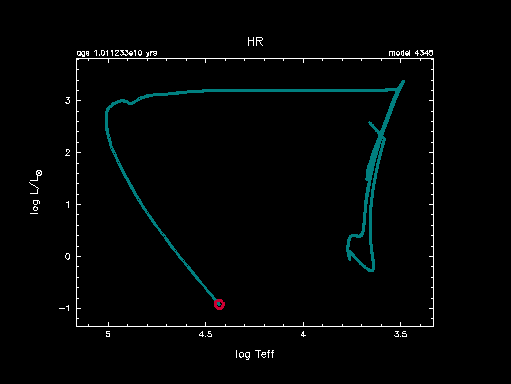
\includegraphics[width=\columnwidth]{1.06_hr_profile.png}
    \caption{H-R Diagram for the 1.06 \(M_\odot\) star model.}
    \label{fig:1.06_Msun_HR_figure}
\end{figure}

A star's luminosity is directly related to its mass and temperature. When discussing a low-mass star, such as the 1.06 \(M_\odot\) modeled, the star's energy is directly proportional to its temperature by $\epsilon \propto T_c$. The H-R diagram allows us to view the evolution of the star in terms of its luminosity and temperature.

The model shows the protostar as it evolves onto the zero-age main sequence (ZAMS). During this time, the temperature is fairly constant, $T_{\text{eff}}$ remained slightly above 3.6, and the luminosity relationship ($L/L_\odot$) has a sharp drop from 2 to -0.5. 

The star then remains on the ZAMS while it continues its hydrogen core burning. As the hydrogen in the core burns, helium is produced. As the stellar core becomes more helium-based and the hydrogen begins to get used up, the density increases, and the core contracts. As the core contracts, the star moves off the ZAMS, and the luminosity ratio increases.

The model showed some surprises as the star moved off the ZAMS. There is a distinct drop in luminosity right before it increases and the temperature shifts back to the right. This was something unexpected to me. I expected to see a smooth transition here.

Once the star moves off the ZAMS, it is considered to be in the subgiant branch. This occurs when the star reaches approximately 2 Gyrs. During this phase, the envelope of the star expands, and the temperature decreases. This is because the core is dense and there is a lot of energy buildup. That energy has to go somewhere, so the core begins to expand. The model demonstrated this stage of evolution unsurprisingly.

At this point, the star has a helium core which is degenerate. The envelope is cool and there is a convective envelope. We call this stage in the evolution of a star the Red Giant Branch (RGB). During the RGB, the structure of the star only depends on the mass of the core. It is independent of temperature. So we see a hydrogen shell causing the core mass to contract slowly. The envelope (and radius) increase and so does the luminosity.

After the red-giant branch, a "Helium Flash" occurs when $M_{\text{core}} \approx 0.45 M_\odot$. The core is unstable (and degenerate) at this stage, and a large volume of helium burns suddenly and all at once. This occurs at $T \approx 10^8$ K. After the main flash, the core expands but remains partially degenerate. Smaller flashes continue to occur for about 1.5 million years.

I was also surprised by the model after the helium flash. The model fluctuates more vertically and less horizontally than I had expected. I was expecting more of a curve rather than a sudden drop.

After the helium flash, the helium burning becomes stable. As the helium burns, the temperature begins to shift right and the luminosity increases again. This process leads the star into the asymptotic giant branch (AGB) phase of its life cycle. It is during this stage that the star begins to develop an iron and carbon core. The AGB phase lasts approximately 100,000 years.

As the star is in the AGB stage, the envelope continues to expand and energy continues to release. When a low-mass star exceeds 30,000 K, the star develops a fast "wind". The UV flux ionizes the gas and a planetary nebula is formed. During this time, the mass of the envelope continues to increase. When $M_{\text{envelope}} \approx 10^{-5} M_\odot$, the hydrogen-burning shell is extinguished. What remains is a degenerate star with $T_{\text{eff}} \approx 10,000 - 15,000$ K, a white dwarf.

The end of the life stages in the 1.06 \(M_\odot\) model was reasonably consistent with my expectations. There was a slight irregularity as the temperature and luminosity dropped off. However, most of the end-stage activity was expected.

\subsection{1.06 \(M_\odot\) Kippenhahn Diagram}

\begin{figure}
    \centering
    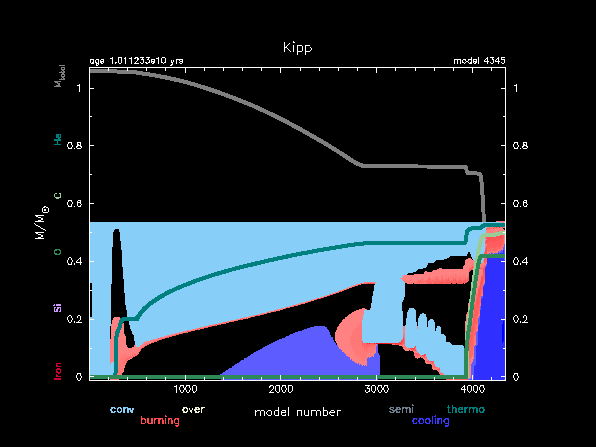
\includegraphics[width=\columnwidth]{1.06_kipp_profile.png}
    \caption{Kipp Diagram for the 1.06 $M_\odot$ star model.}
    \label{fig:1.06_Msol_kipp_figure}
\end{figure}


\par The kippenhahn diagram tells a lot about what is happening in the interior of the star. The x-axis represents the age of the star in (Myrs).  The y-axis provides the mass of the star. As the star begins its life cycle it is entirely convective core burning.  The light blue represents the convective core burning and we can see the max mass of the star being represented as a greyish line above.  For example $ M_{star} \approx 1.6 $, the core is fully convective (light blue) between 0M and 0.5M on the far left of the graph. 

\par As the core becomes more $ He_{core} $and the temperature increases, the core changes from convective to radiative.  We say that it is now "core burning." We see this core burning begin as a red representation on the graph.  However, what is also interesting about the diagram is that there is degeneracy in the core above the radiative section. 

\par As the star approaches the Helium flash the core is becoming increasingly degenerate.  This is shown in the diagram by the black spaces at the bottom of the graph.  This degeneracy is expected because the core is in the sub-giant and red-giant branches.  Notice also that the overall mass of the star is decreasing steadily.  This is because the star is burning the "fuel" and using energy.

\par We also see core cooling happening in this diagram. There is cooling that occurs inside the core when there is shell burning.  This diagram shows that there is convective shell burning, degeneracy, and core cooling at the midpoint of the diagram. 
\par As the overall mass decreases, there is an increase in density and this causes ignition in the core again.  So we get a radiative spike towards the end of the core cooling. the convective shell also reacts and there is convection in the layers above the radiation.
\par As the star moves into the AGB and nebula cycles the convection and radiation continue in specified areas of the star.  However, we see the mass of the star compress quickly and there is a spike in the cooling of the star simultaneously. Most of the convection at this point has dissipated and there is a small amount of radiation left.  This point signifies the creation of the white dwarf.

\subsection{1.06 \(M_\odot\) TRHO Profile}

\begin{figure}
    % To include a figure from a file named example.*
    % Allowable file formats are eps or ps if compiling using latex
    % or pdf, png, jpg if compiling using pdflatex

    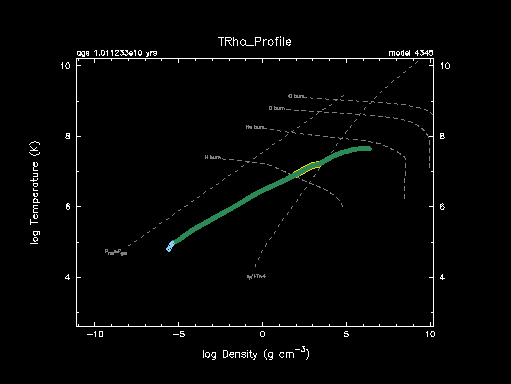
\includegraphics[width=\columnwidth]{1.06_trho_profile.png}
    \caption{TRHO Profile for the 1.06 $M_\odot$ star model.}
    \label{fig:1.06_Msol_trho_figure}
\end{figure}


\par To conclude the 1.06\(M_\odot\) I plotted a Temperature vs Density profile (Trho profile).  What I found most interesting about this diagram was the almost linear relationship between the two. The star continued to increase in density over the duration of its lifespan, even though the overall radius of the star expands as the envelope expands.  We know this to be true, but this profile helps confirm that.  But the relation of the temperature was surprising.
\par Although the profile starts out as convective, the majority of the profile is "non-mixing," which is represented as green.  There is also a potion of the profile when density is between 1.5 and 3.5 that we see that there is $ > 1 erg* g^{-1}s^{-1}$. 

\section{5.06 \(M_\odot\) star and the Stellar Evolution for a Mid Mass Star}
I used a 5.06 \(M_\odot\) star to plot a stellar evolution model of a larger-sized star. I wanted to simulate a realistic star and the parameters of the project required $ [Fe/H]=0 $.  I set the metalicity to reflect those parameters with the knowledge that I would run the same model again with a different metallicity later in the research. The largest surprise I saw in this model was the sudden stop of the H-R diagram.  This time the diagram did not show the star moving into the nebula or white dwarf stage of its evolution.


\subsection{5.06 \(M_\odot\) H-R Diagram}
% H-R Diagram 1.0

\begin{figure}
    % To include a figure from a file named example.*
    % Allowable file formats are eps or ps if compiling using latex
    % or pdf, png, jpg if compiling using pdflatex

    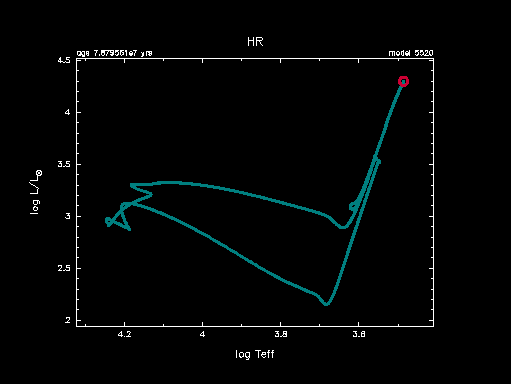
\includegraphics[width=\columnwidth]{hr_profile_05520.png}
    \caption{H-R Diagram for the 5.06 \(M_\odot\) star model.}
    \label{fig:5.06_M_sun_HR_figure} % Correct placement of \label
\end{figure}

\par We expect a very similar process for any protostar moving onto the ZAMS (Zero-Age Main Sequence). The diagram shows a nearly vertical drop in luminosity as the star evolves onto the ZAMS. Once on the ZAMS, there is a strong linear relationship between temperature and luminosity. Stars with \(M > 1.3 M_\odot\) use the CNO cycle, whereas lower mass stars use the P-P Chain. This implies that we will observe some differences in the evolution of this star compared to the star observed earlier in the paper.

\par Stars with \(0.35 M_\odot < M < 1.2 M_\odot\) have a core that is both radiative and convective. This results in their gradual movement off the ZAMS. However, for stars with \(M > 1.2 M_\odot\), the core is completely convective, and the helium core is non-degenerate. Consequently, helium ignition is stable and allows for steady helium burning, preventing a helium flash. When hydrogen is exhausted, there is a sudden drop in temperature, but the luminosity remains constant, resulting in a sharp "hook-like" feature on the diagram. This typically occurs when the metallicity mass fraction is about 0.03 in the core and marks the beginning of the overall contraction phase.

\par The diagram displays some interesting movements just before the hook. As the star moves off the ZAMS, there is a decrease in both luminosity and temperature. The graph then quickly changes direction, increasing at a shallow pace before spiking into a steep slope leading to the hook.

\par Shell burning occurs at the end of the hook, where hydrogen in the core is exhausted, leading to the disappearance of a convective core. This stage lasts approximately \(10^5\) years. During this phase, the core contracts, the envelope expands, and luminosity decreases. This part of stellar evolution is known as the "Hertzsprung Gap."

\par The increase in the envelope radius, decrease in temperature, and increase in opacity lead to convection within the star. A significant portion of the envelope becomes convective. With a convective envelope, the core contracts further, causing the envelope to expand more. Energy is transferred through convection, meaning the temperature remains constant. The only way for energy to be transferred is for the luminosity to spike, leading to the "Red-Giant Branch" (RGB) phase of the star's evolution.

\par The H-R Diagram shows the RGB spike very clearly. Aside from the previously mentioned motion coming off the ZAMS, it aligns well with expectations. The hook feature is very pronounced on the left side of the diagram, and the RGB is distinct on the right.

\par Following the RGB phase, stars with \(M \approx 0.6 M_\odot\) and \(T_{eff} \approx 10^8 \text{K}\) undergo helium ignition in a non-degenerate core. The stable helium burning halts any further core contraction, causing the envelope to stop expanding. The core becomes convective once again, and the process involves a \(3\alpha\) reaction. This stage can last approximately 22 Myrs.

\par I was surprised by this stage of evolution when observing the diagram. This stage appears juxtaposed with the RGB phase, blending together and making it seem as though they are the same. However, multiple stages occur on the same slope.

\par After helium ignition, the core contracts, the radius decreases, and luminosity drops. At this point, the envelope is radiative, and the star leaves the giant branch (although it doesn’t seem to have completely "left" the giant branch). When \(Y \approx 0.3\), the core is undergoing helium burning. When \(Y > 0.5\), the envelope begins to expand again. The star then moves back onto the giant branch and the Hayashi Line.

\par This transition occurs when \(M_{core} \approx 0.6 M_\odot\) and \(T \approx 10^8 \text{K}\). The core remains non-degenerate, and helium ignition halts further core contraction.

\par I expected the model to continue with the star's evolution, eventually progressing to the AGB stage, evolving into a planetary nebula, and eventually becoming a white dwarf. However, the model stopped at the point where core contraction ceased, which was my biggest surprise of all the models.


\subsection{5.06 \(M_\odot\) Kippenhahn Diagram}

\begin{figure}
    % To include a figure from a file named example.*
    % Allowable file formats are eps or ps if compiling using latex
    % or pdf, png, jpg if compiling using pdflatex

    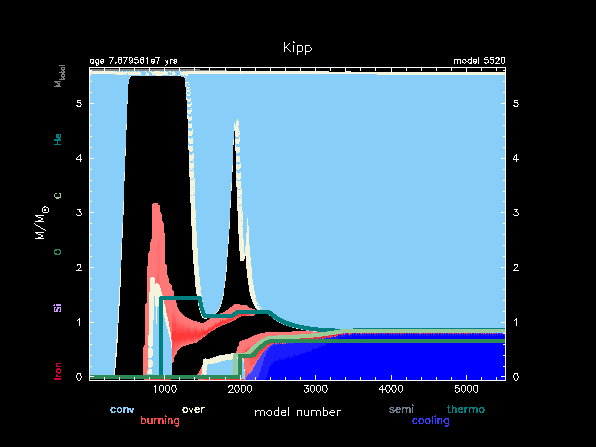
\includegraphics[width=\columnwidth]{kipp_profile05520.png}
    \caption{Kippenhahn Diagram for the 5.06 \(M_\odot\) star model.}
    \label{fig:5.06_M_sun_kipp_figure}
\end{figure}

\par The Kippenhahn diagram for the 5.06 \(M_\odot\) star model illustrates much of what was discussed in the previous section. We know that a \(5.06 M_\odot\) star has a convective core that burns consistently. This is clearly evident at the beginning of the diagram. As mentioned earlier, the exhaustion of hydrogen causes convection to disappear in the core during the "hook feature." The diagram shows the disappearance of convection (blue) around the expected time. There is some radiative activity in the core and a small amount of convection that was not fully anticipated, but this aligns with diagrams from lectures showing the hydrogen and helium burning stages.

\par At the end of the Kippenhahn diagram, we observe the cooling stage of the core. Since the core is no longer gaining density, we do not expect its temperature to increase. As energy dissipates, the core cools down.

\subsection{5.06 \(M_\odot\) TRHO Profile}

\begin{figure}
    % To include a figure from a file named example.*
    % Allowable file formats are eps or ps if compiling using latex
    % or pdf, png, jpg if compiling using pdflatex

    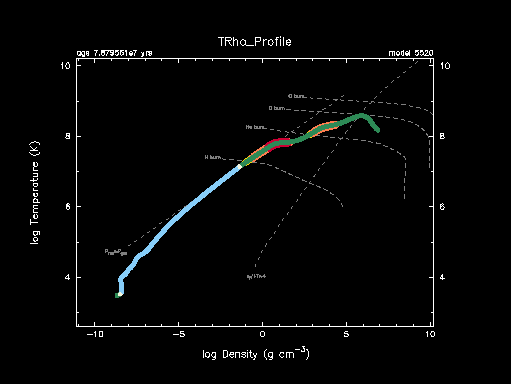
\includegraphics[width=\columnwidth]{trho_profile_05520.png}
    \caption{TRHO Profile for the 5.06 \(M_\odot\) star model.}
    \label{fig:5.06_M_sun_trho_figure}
\end{figure}

\par I expected the TRHO profile for the \(5.06 M_\odot\) star to show more convection, given that more massive stars are expected to exhibit convective burning, which is the basis for the hook feature. The profile indeed shows convection in the initial part of the diagram. The relationship between temperature and density is similar to the first model but with a slightly different curvature. The graph displays more yellow areas representing \(> 1 \text{ erg} \cdot \text{g}^{-1} \text{s}^{-1}\), and introduces red regions indicating \(> 10^7 \text{ erg} \cdot \text{g}^{-1} \text{s}^{-1}\).


\section{Metallicity and the Effects it has on the evolution of 5.06 \(M_\odot\) stars}
For this section, the assignment wanted $[Fe/H] = -1$.  Since the chemical abundance is in log space, and the difference from 0 to -1 is a factor of $10^{-1}$, I was able to set $Z=0.02$.  This was a similar value that I used for the low-mass star, which made me curious to see how the higher-mass star looked.

\begin{figure}
	% To include a figure from a file named example.*
	% Allowable file formats are eps or ps if compiling using latex
	% or pdf, png, jpg if compiling using pdflatex

	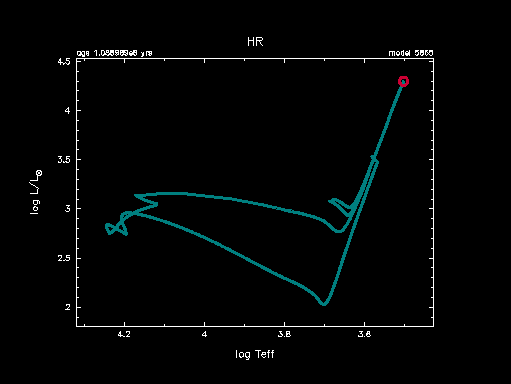
\includegraphics[width=\columnwidth]{hr_profile_05865.png}
    \caption{HR Profile for the 5.06 $M_\odot$ (0.02) star model.}
    \label{fig:5.06_Msol_0.02_hr_figure}
\end{figure}



\subsection{5.06 \(M_\odot\) H-R Diagram Comparison}
\par The most noticeable difference between the two diagrams is that the lower metalicity star has a distinct $H_{core}$ burning phase.  This time it is not juxtaposed to the RGB and AGB phases. My best explanation for this is that since there is less metalicity in the modified profile, there is more Hydrogen to burn in the core.  So the Core Hydrogen burning phase is going to be stronger and create a greater temperature increase.

\par Other observations between these two diagrams include a steeper slope of the graph after the hydrogen shell burning starts (following the hook feature).  As well as a less distinct line coming off the ZAMS.
\par It is worth mentioning that the star's end behavior remains the same. Even when changing the metalicity in such a way, the star still went through the same phases and died in the same manner.
\subsection{5.06 \(M_\odot\) Kippenhahn Diagram Comparison}

\begin{figure}
    \centering
    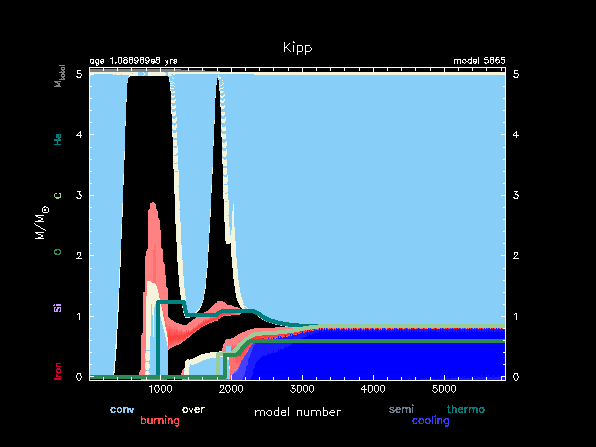
\includegraphics[width=\columnwidth]{kipp_profile05865.png}
    \caption{Kipp Profile for the 5.06 $M_\odot$ (0.02) star model.}
    \label{fig:5.06_Msol_0.02_kipp_figure}
\end{figure}



\par The Kippenhahn diagrams are almost identical.  The largest difference I see is that the modified model has a much greater degeneracy factor after the second convective core burning stage.  During the $H_{core}$ burning phase there is a $3\alpha$ reaction and we should see a convective core. The degeneracy is occurring above this convective core. Therefore I believe that this degeneracy is occurring at the same time as the discrepancy we saw on the H-R diagrams. 
\subsection{5.06 \(M_\odot\) TRHO Diagram Comparison}
\par When evaluating the two temperature vs density plots, it does not appear that there is not any noticeable discernment. Certainly, not any of the merit that would make a significant difference. However, I think that, in itself, is worth noting. This implies that the temperature and density of the star are independent of metalicity. I am not convinced that it is true, however, it is something worth considering and studying further.

\begin{figure}
    \centering
    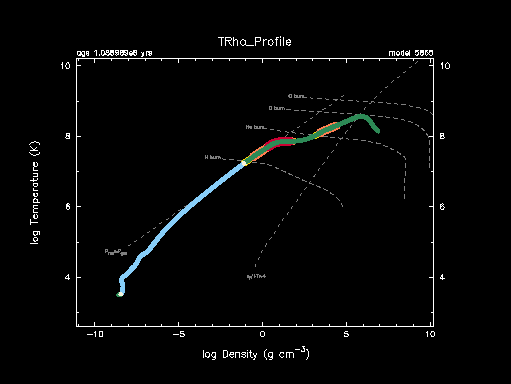
\includegraphics[width=\columnwidth]{trho_profile_05865.png}
    \caption{TRHO Profile for the 5.06 $M_\odot$ (0.02) star model.}
    \label{fig:5.06_Msol_0.02_trho_figure}
\end{figure}



\section{50.6 \(M_\odot\) Star and Stellar Evolution for a High-Mass Star}

I decided to model a \(50.6 M_\odot\) star for the high-mass star category. The choice of this value was somewhat arbitrary; it met the criteria of the assignment, so I simply scaled the 5.06 \(M_\odot\) model by a factor of ten. This specific model proved to be quite predictable, with few surprises during its execution.


\subsection{50.6 \(M_\odot\) H-R Diagram}

\begin{figure}
    \centering
    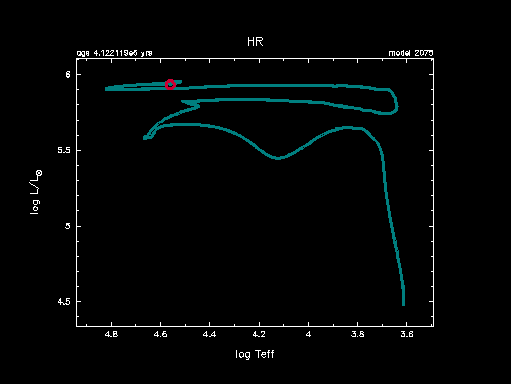
\includegraphics[width=\columnwidth]{50.6 HR.png}
    \caption{H-R Diagram for the \(50.6\ M_\odot\) star model.}
    \label{fig:50.6_Msol_hr_figure}
\end{figure}


\par For very massive stars, we need to consider the Humphreys-Davidson (H-D) Limit. Stars with \(M > 40 M_\odot\) do not become red supergiants due to this limit. Instead, such luminous stars are known as Luminous Blue Variables (LBVs), which are related to Wolf-Rayet stars. Despite this, the evolution of more massive stars up to the giant branch is similar to that of mid-sized stars. Therefore, I expected to see a hook feature and other familiar characteristics in this model's H-R Diagram.

\par The hook feature appears at higher temperatures and luminosities, as expected, and is clearly visible. Additionally, I anticipated a sharp curve to the left as temperature increased. The model exhibits an almost horizontal shift, suggesting that the upper limits of the graph are close to the H-D Limit. The core mass is so large that it ignites carbon, which burns and converts to iron. This process can take up to 1,000 years. Since the core mass remains relatively stable, the envelope does not have time to adjust, resulting in a fixed position on the H-R Diagram beyond carbon burning.

\subsection{50.6 \(M_\odot\) Kippenhahn Diagram}

\par The Kippenhahn diagram for the \(50.6 M_\odot\) star was the most unusual. I expected to see more convective burning in the core at the beginning. However, the plots suggest that the base of the core is radiative with degeneracy and only a small amount of convection in the middle. The reason for this initial configuration is unclear, but eventually, as expected, the core exhibits convection.

\par There is a sudden mass decrease early in the star's life cycle, which is anticipated as the star approaches the H-D Limit. Following this, there is a mixture of cooling and radiative activity, but the majority of the star remains convective. This outcome aligns with expectations. Several convective shell-burning episodes occur during this stage, and the number of these shells influences the final outcome of the star's core mass.

\begin{figure}
    \centering
    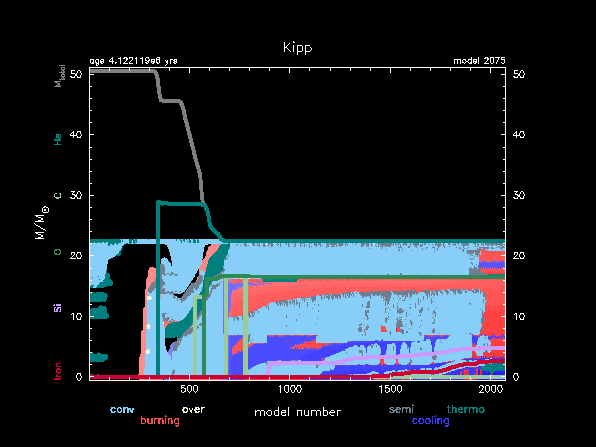
\includegraphics[width=\columnwidth]{50.6 kipp.png}
    \caption{Kippenhahn Diagram for the \(50.6\ M_\odot\) star model.}
    \label{fig:50.6_Msol_kipp_figure}
\end{figure}



\subsection{50.6 \(M_\odot\) TRHO Profile}

\begin{figure}
    \centering
    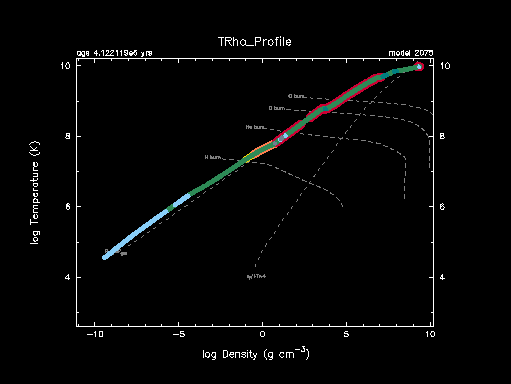
\includegraphics[width=\columnwidth]{50.6 Trho.png}
    \caption{TRHO Profile for the \(50.6\ M_\odot\) star model.}
    \label{fig:50.6_Msol_trho_figure}
\end{figure}



\par As with most of the other profiles, we see a strong convective core beginning.  This can be attributed to the size of the larger stars and the CNO process.  Also, similar to the other the star shows a green "no mixing" section.  The profile starts to change from this point on.  It shows similar yellow lines, $ > 1 erg* g^{-1}s^{-1}$, as well as the red lines,$ > 10^{7} erg* g^{-1}s^{-1}$.  In addition to these lines, this profile also shows orange lines representing $ > 1000 erg* g^{-1}s^{-1}$
\par The plot is still linear, but it differs from the other plots in that it extends much further.  It has a higher temperature and density. This is not surprising since it is a more massive star.
\section{Conclusions}

The majority of the plots and graphs from the four different models were overall consistent with the expectations.  Based on the information we learned in class this year and the outlines that were shown in class and found through the texts, these models are appropriately run. Although this paper did not completely compare the models as they relate to each other in time, we did look at where the models were in comparison to the stages of evolution.  This allowed us to see the similarities between topics, like shell and core burning, from the kippenhahn diagrams with the luminosity and temperature relations on the H-R diagram.
\par It also is very interesting to see how metalicity impacts the evolution and life cycle of stars. Changing a star's overall makeup can give it a very different look.  However, we noticed that there were little effects of the density, temperature, and end behavior of the star when we changed the metalicity.
\par Although there are more items that can be analyzed and some questions remain that I was not fully able to answer, these models are great examples to help gain understanding and insight into the mystery of stellar evolution.

\section*{Acknowledgements}

I would like to give a special thanks to Chanuntorn Pumpo for her help in evaluating the Metalicity of $[Fe/H]=-1$.  Tucker Capps, Ryan Abbott, Megan Firgard, Simon Lowry, Emily Tipton, Sean Smith, and Wes Thiels for their continued help and support during this and other projects.

%%%%%%%%%%%%%%%%%%%%%%%%%%%%%%%%%%%%%%%%%%%%%%%%%%
\section*{Data Availability}

 All relevant files and outputs are located in \url{/home/john0716/Stellar_Final_Project/} on the university computers.

\section*{References}
\par Kilic, Mukremin. “The Evolution of Stars” Class lecture, Astro 3103,
University of Oklahoma, Norman Oklahoma, Fall, 2021
\par Kilic, Mukremin. “Stellar Evolution” Class lecture, Astro 4303,
University of Oklahoma, Norman Oklahoma, Fall, 2022
\par Kilic, Mukremin. “Stellar Evolution” Class lecture, Astro 4303,
University of Oklahoma, Norman Oklahoma, Fall, 2022
\par Carroll, Bradley W., and Dale A. Ostlie. An Introduction to Modern Astrophysics. Cambridge University Press, 2021. 
\par Kippenhahn, Rudolf, et al. Stellar Structure and Evolution. Springer, 2020. 
\par LeBlanc, Francis. An Introduction to Stellar Astrophysics. Wiley, 2010. 

%%%%%%%%%%%%%%%%%%%% REFERENCES %%%%%%%%%%%%%%%%%%

% The best way to enter references is to use BibTeX:

%\printbibliography %Prints bibliography


% Alternatively you could enter them by hand, like this:
% This method is tedious and prone to error if you have lots of references
%\begin{thebibliography}{99}
%\bibitem[\protect\citeauthoryear{Author}{2012}]{Author2012}
%Author A.~N., 2013, Journal of Improbable Astronomy, 1, 1
%\bibitem[\protect\citeauthoryear{Others}{2013}]{Others2013}
%Others S., 2012, Journal of Interesting Stuff, 17, 198
%\end{thebibliography}

%%%%%%%%%%%%%%%%%%%%%%%%%%%%%%%%%%%%%%%%%%%%%%%%%%

%%%%%%%%%%%%%%%%% APPENDICES %%%%%%%%%%%%%%%%%%%%%

%\appendix

%\section{Some extra material}

%If you want to present additional material which would interrupt the flow of the main paper,
%it can be placed in an Appendix which appears after the list of references.

%%%%%%%%%%%%%%%%%%%%%%%%%%%%%%%%%%%%%%%%%%%%%%%%%%


% Don't change these lines
\bsp	% typesetting comment
\label{lastpage}
\end{document}

% End of mnras_template.tex